\documentclass{beamer}
%\usetheme{Boadilla}
%\usetheme{Szeged}
%\usetheme{Singapore}
\usetheme{Frankfurt}
\usecolortheme{dove}
\setbeamertemplate{navigation symbols}{}
\setbeamertemplate{headline}{}
\setbeamertemplate{footline}[text line]{\parbox{\linewidth}{\vspace*{-8pt}\insertsectionnavigationhorizontal{.95\paperwidth}{\hspace{-32pt}}{\hfill\hfill}}}

\newenvironment{alltt}{\ttfamily}{\par}
\usepackage{amsmath,amssymb,amsfonts,amsthm, multicol, subfigure, color}
\usepackage{bm}
\usepackage{graphicx}
\usepackage{tabularx}
\usepackage{booktabs}
\usepackage{hyperref}
\usepackage{pdfpages}
\definecolor{dodgerblue}{rgb}{.118, .575, 1}
\def\independenT#1#2{\mathrel{\rlap{$#1#2$}\mkern2mu{#1#2}}}
\newcommand\independent{\protect\mathpalette{\protect\independenT}{\perp}}
\newcommand\indep{\protect\mathpalette{\protect\independenT}{\perp}}
\def\logit{\text{logit}}
\usepackage{stackrel}
\usepackage{tikz}
\usetikzlibrary{arrows,shapes.arrows,positioning,shapes}
\newcommand\red[1]{{\color{red}#1}}
\newcommand\bred[1]{{\color{red}\textbf{#1}}}
\newcommand\blue[1]{{\color{blue}#1}}
\newcommand\bblue[1]{{\color{blue}\textbf{#1}}}
\newcommand\green[1]{{\color{olive}#1}}
\newcommand\bgreen[1]{{\color{olive}\textbf{#1}}}
\newcommand\purple[1]{{\color{purple}#1}}
\newcommand\orange[1]{{\color{orange}#1}}
\newcommand\black[1]{{\color{black}#1}}
\newcommand\white[1]{{\color{white}#1}}
\newcommand\teal[1]{{\color{teal}#1}}
\newcommand\magenta[1]{{\color{magenta}#1}}
\newcommand\Fuchsia[1]{{\color{Fuchsia}#1}}
\newcommand\BlueGreen[1]{{\color{BlueGreen}#1}}
\newcommand\iid{\stackrel{\text{iid}}{\sim}}
\newcommand\E{\text{E}}
\newcommand\V{\text{V}}
\renewcommand\P{\text{P}}
\newcommand{\tcframe}{\frame{
\small{
\only<1|handout:0>{\tableofcontents}
\only<2|handout:1>{\tableofcontents[currentsection]}}
}}
% Credit for the following to https://tex.stackexchange.com/questions/44983/beamer-removing-headline-and-its-space-on-a-single-frame-for-plan-but-keepin
\makeatletter
    \newenvironment{withoutheadline}{
        \setbeamertemplate{headline}[default]
        \def\beamer@entrycode{\vspace*{-\headheight}}
    }{}
\makeatother
\setbeamercovered{invisible}

\newcommand{\goalsframe}{\begin{frame}{Learning goals for today}
By the end of class, you will be able to
\begin{itemize}
    \item make assumptions about missing data
    \begin{itemize}
    \item missing completely at random
    \item missing at random
    \end{itemize}
    \item connect these assumptions to causal inference
    \item use two strategies for missing data
    \begin{itemize}
    \item listwise deletion
    \item multiple imputation
    \end{itemize}
 \end{itemize} 
  \vskip .2in
\end{frame}}

\title{Missing Data}
\subtitle{Soc 212C}
\author{Ian Lundberg}
\date{}

\begin{document}

\frame{\titlepage}

\goalsframe

\section{Motivation}

\begin{frame}
\begin{multicols}{2}
\includegraphics[width = .5\textwidth]{figs/Abraham_Wald}\footnote{PC: Wikimedia commons}

Abraham Wald 
\begin{itemize}
\item b. 1902, Austria-Hungary
\item Jewish, persecuted in WWII
\item Fled to U.S. in 1938
\item Namesake of the Wald test
\item Statistical consultant for U.S. Navy in WWII
\end{itemize}
\end{multicols}
\end{frame}

\begin{frame}
\textcolor{blue}{Question:} Where should armor be added to protect planes? \vskip 1cm
\textcolor{blue}{Data:} Suppose we saw the following planes.\footnote{Story told by Mangel and Samaniego 1984 [\href{http://dx.doi.org/10.1080/01621459.1984.10478038}{\textcolor{blue}{link}}].\\ Presentation style inspired by Joe Blitzstein. See the original here [\href{https://www.youtube.com/watch?v=dzFf3r1yph8}{\textcolor{blue}{link}}] \vskip .2cm}
\end{frame}

\begin{frame}{\blue{Observed data}: Planes that came home with damage}
\begin{center}
\begin{tikzpicture}[x = .5\textwidth, y = .5\textheight]
\node at (0,0) {\includegraphics[width = .6\textwidth]{figs/planes.jpg}};
% Upper left plane (tail hits)
\onslide<2->{\node at (-.4,.35) {\huge \red{$\bullet$}};}
\onslide<3->{\node at (-.45,.3) {\huge \red{$\bullet$}};}
\onslide<4->{\node at (-.5,.33) {\huge \red{$\bullet$}};}
\onslide<5->{\node at (-.55,.28) {\huge \red{$\bullet$}};}
\onslide<6->{\node at (-.53,.4) {\huge \red{$\bullet$}};}
\onslide<7->{\node at (-.3,.3) {\huge \red{$\bullet$}};}
% Upper right plane (one wing hits)
\onslide<9->{\node at (.1,.35) {\huge \red{$\bullet$}};}
\onslide<10->{\node at (.3,.35) {\huge \red{$\bullet$}};}
\onslide<11->{\node at (.25,.28) {\huge \red{$\bullet$}};}
\onslide<12->{\node at (.4,.25) {\huge \red{$\bullet$}};}
\onslide<13->{\node at (.32,.21) {\huge \red{$\bullet$}};}
\onslide<14->{\node at (.32,.1) {\huge \red{$\bullet$}};}
% Lower left plane (body and one wing hits)
\onslide<15->{\node at (-.3,-.3) {\huge \red{$\bullet$}};}
\onslide<16->{\node at (-.5,-.3) {\huge \red{$\bullet$}};}
\onslide<17->{\node at (-.35,-.25) {\huge \red{$\bullet$}};}
\onslide<18->{\node at (-.4,-.27) {\huge \red{$\bullet$}};}
\onslide<19->{\node at (-.28,-.2) {\huge \red{$\bullet$}};}
\onslide<20->{\node at (-.3,-.1) {\huge \red{$\bullet$}};}
% Lower right plane (body hits)
\onslide<21->{\node at (.1,-.3) {\huge \red{$\bullet$}};}
\onslide<22->{\node at (.25,-.23) {\huge \red{$\bullet$}};}
\onslide<23->{\node at (.2,-.3) {\huge \red{$\bullet$}};}
\onslide<24->{\node at (.32,-.28) {\huge \red{$\bullet$}};}
\node at (0,-.8) {\Large \blue{Q:} Where would you add armor?};
\end{tikzpicture}
\end{center}
%Where should we add armor?
\end{frame}

\begin{frame}{\blue{Missing data}: Planes that never returned}
\pause
\begin{center}
\begin{tikzpicture}[x = .5\textwidth, y = .5\textheight]
\node at (0,0) {\includegraphics[width = .6\textwidth]{figs/planes.jpg}};
% Upper left plane
\node at (-.09,.34) {\huge \red{$\bullet$}};
\node at (-.14,.3) {\huge \red{$\bullet$}};
% Upper right plane
\node at (.53,.31) {\huge \red{$\bullet$}};
\node at (.47,.33) {\huge \red{$\bullet$}};
% Lower left plane
\node at (-.09,-.25) {\huge \red{$\bullet$}};
\node at (-.14,-.25) {\huge \red{$\bullet$}};
% Lower right plane
\node at (.53,-.25) {\huge \red{$\bullet$}};
\node at (.48,-.27) {\huge \red{$\bullet$}};
\end{tikzpicture}
\end{center}
\end{frame}

\begin{frame}
\large We should add armor to the nose! \vskip 1cm
The missing planes are unlike the observed planes.\\
Requires argument---no algorithm has the answer.
\end{frame}

\section{Concrete Example}

\begin{frame}{Missing data in social science}

Any NA in your dataset is like a plane that never returned. \vskip .2in
It requires careful thought, not a one-size-fits-all procedure.

\end{frame}


\begin{frame}[t]{A concrete example}

What is the employment rate among these 6 people? \vskip .2in

\begin{center}
\begin{tabular}{llll}
HS graduate? & Employed? & Missing? & \\
$X$ & $Y_\text{True}$ & $M_Y$ & $Y_\text{Observed}$ \\
\hline
1 & 0 & 0 & 0 \\
1 & 1 & 0 & 1 \\
1 & 0 & 1 & NA \\
1 & 1 & 1 & NA \\
0 & 0 & 0 & 0 \\
0 & 0 & 0 & 0 \\
\hline
\end{tabular}
\end{center}

$$
\begin{aligned}
&\text{Truth} & \frac{2}{6} = \frac{1}{3} \\ \pause
&\text{Estimate dropping NA}\qquad & \frac{1}{4} \\
%&\text{Estimate within $X$} & \frac{4\times \frac{1}{2} + 2\times\frac{0}{2}}{6} = \frac{1}{3}
\end{aligned}
$$

\end{frame}

\section{MCAR Assumption}

\begin{frame}{Missing completely at random and listwise deletion}

If $\{M_X,M_Y\} \indep \{X,Y\}$, then you can simply drop missing cases. \vskip .2in
\begin{itemize}
\item This approach is called listwise deletion
\item This assumption is called missing completely at random
\item Assumption did not hold in this case
\end{itemize}

\end{frame}

\section{MAR Assumption}

\begin{frame}{Missing at random: Listwise deletion within $X$}

What if we assume $Y\indep M_Y\mid X$?

\begin{center}
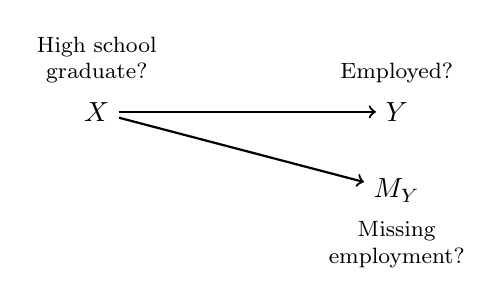
\begin{tikzpicture}[x = 1.5in]
\node (x) at (0,0) {$X$};
\node (my) at (1,-1) {$M_Y$};
\node (y) at (1,0) {$Y$};
\draw[->, thick] (x) -- (my);
\draw[->, thick] (x) -- (y);
\node[anchor = south, font = \footnotesize, align = center] at (x.north) {High school\\graduate?};
\node[anchor = south, font = \footnotesize, align = center] at (y.north) {Employed?};
\node[anchor = north, font = \footnotesize, align = center] at (my.south) {Missing\\employment?};
\end{tikzpicture}
\end{center}

Then we can estimate $E(Y)$ by adjusting for $X$.

\end{frame}

\begin{frame}{Missing at random: Listwise deletion within $X$}

$$
\begin{aligned}
E(Y) &= \E(Y\mid X = \text{HS graduate}) \times \P( X = \text{HS graduate}) \\
&\qquad + \E(Y\mid X \neq \text{HS graduate}) \times \P( X \neq \text{HS graduate}) \\
{}\\
&= \E(Y\mid X = \text{HS graduate}, M_Y = 0) \times \P( X = \text{HS graduate}) \\
&\qquad + \E(Y\mid X \neq \text{HS graduate}, M_Y = 0) \times \P( X \neq \text{HS graduate}) \\
{} \\
&= \frac{1}{2} \times \frac{4}{6} + 0\times\frac{2}{6} \\
&= \frac{1}{3}
\end{aligned}
$$

\end{frame}

\begin{frame}{Missing at random: Imputation}

\begin{center}
\begin{tabular}{lllll}
HS graduate? & Employed? & Missing? & \\
$X$ & $Y_\text{True}$ & $M_Y$ & $Y_\text{Observed}$ & $Y_\text{Imputed}$ \\
\hline
1 & 0 & 0 & 0 & 0 \\
1 & 1 & 0 & 1 & 1\\
1 & 0 & 1 & NA & 0.5 \\
1 & 1 & 1 & NA & 0.5 \\
0 & 0 & 0 & 0 & 0 \\
0 & 0 & 0 & 0 & 0 \\
\hline
\end{tabular}
\end{center} \vskip .2in
Exactly like causal inference:\\
when $Y$ is not observed, impute its value under assumptions.

\end{frame}

\section{Multivariate Missingness}

\begin{frame}{Generalizing to multivariate missingness}

We hope for missing at random\hfill 
$M_X\indep X\mid Y$ and $M_Y\indep Y\mid X$
\vskip .1in
\begin{center}
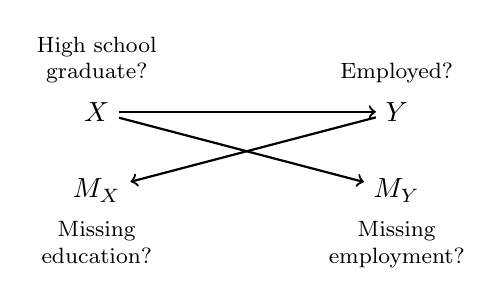
\begin{tikzpicture}[x = 1.5in]
\node (x) at (0,0) {$X$};
\node (mx) at (0,-1) {$M_X$};
\node (my) at (1,-1) {$M_Y$};
\node (y) at (1,0) {$Y$};
\draw[->, thick] (x) -- (my);
\draw[->, thick] (x) -- (y);
\draw[->, thick] (y) -- (mx);
\node[anchor = south, font = \footnotesize, align = center] at (x.north) {High school\\graduate?};
\node[anchor = south, font = \footnotesize, align = center] at (y.north) {Employed?};
\node[anchor = north, font = \footnotesize, align = center] at (my.south) {Missing\\employment?};
\node[anchor = north, font = \footnotesize, align = center] at (mx.south) {Missing\\education?};
\end{tikzpicture}
\end{center}
\vskip .1in
More generally, we hope \hfill $\vec{M}\indep \text{Data}_\text{Missing}\mid\text{Data}_\text{Observed}$

\end{frame}

\section{Standard Errors}

\begin{frame}{Standard errors by the bootstrap}
Use the estimator function $s()$
\begin{itemize}
\item Point estimate $\hat\tau = s(\text{data})$
\item Bootstrap confidence interval by quantiles of $s(\text{data}^*)$
\end{itemize}
\vskip .2in
Within $s()$
\begin{itemize}
\item impute missing values
\item carry out analysis
\item return estimate
\end{itemize}
\end{frame}

\begin{frame}{Standard errors by math}{Approach is called Rubin's Rules}

Create $m$ imputed datasets.\\
Variance estimator involves variance
\begin{itemize}
\item[--] \bgreen{within} each imputation and 
\item[--] \bblue{between} imputations.
\end{itemize} \pause
\begin{center}
\begin{tikzpicture}[x = .5\textwidth, y = .5\textheight]
\node at (0,0) {$\hat\V(\hat\theta) = \underbrace{\frac{1}{m}\sum_{i=1}^m \hat\V(\hat\theta_i)}_{\substack{\text{Mean}\\\text{\bgreen{within-imputation} variance}}} + \underbrace{\left(1 + \frac{1}{m}\right)}_{\substack{\text{Inflation}\\\text{factor}}}\underbrace{\left(\frac{1}{m-1}\sum_{i=1}^m\left[\hat\theta_i - \bar{\hat\theta}\right]^2\right)}_\text{\bblue{Between-imputation} variance}$};
\end{tikzpicture}
\end{center}

\end{frame}

\section{Closing}

\begin{frame}{What happens in practice}
\begin{itemize}
\item Many variables in $\vec{X}$
\item Swiss cheese missingness
\item Very hard to make assumptions credible
\item Reviewers prefer multiple imputation
\end{itemize}
\end{frame}

\begin{frame}{My advice for dropping cases}
Track dropped cases in a logical order
\begin{itemize}
\item drop outside target population \hfill (non-controversial)
\item drop missing confounder values \hfill (mostly ok)
\item drop missing treatment values \hfill (analogous to ATT)
\item drop missing outcomes \hfill (very dubious)
\end{itemize}
\end{frame}

\begin{frame}{My own workflow}{No guarantees here; my workflow is uncommon.}

I use the \href{https://cran.r-project.org/web/packages/Amelia/index.html}{\textcolor{blue}{\texttt{Amelia}}} package because it is fast. \vskip .1in
\begin{itemize}
\item Write an \texttt{estimator()} function
\begin{itemize}
\item goes from data to an estimate
\item internally calls \texttt{amelia()} to impute
\item set \texttt{boot.type = FALSE} within \texttt{amelia()}\\(bootstrap will be handled separately)
\end{itemize}
\item Use \texttt{estimator(data)} to make a point estimate
\item Bootstrap to make a confidence interval by quantiles of $\texttt{estimator(data}^*\texttt{)}$
\end{itemize}
Here is an \href{https://github.com/ilundberg/replication/blob/780ade188d7fbcdd2d49dc5b3d2c427b31e876ac/gap\_closing\_estimand/code/b\_example\_analyzeData.R\#L94}{\textcolor{blue}{example}} from my code.
\end{frame}

\goalsframe

\end{document}

